%!TEX root = ../username.tex
\chapter{Real Acoustic Spaces}
\hspace*{-0.15cm}This chapter will cover impulse responses and their use in artificial reverberation. It will begin with the mathematical background of rooms and how their echo is measured. Next, several methods of measuring a room's impulse response will be discussed. Finally, the measurements taken from an acoustic space will be provided and the results analyzed.

\section{Mathematical Background}
With the previously mentioned algorithm, it comes naturally that one will need the impulse response of a room in order to have something to convolve with. While several can be found online, measuring the the impulse response from a real acoustic space can provide a baseline to evaluate other methods in a unique and novel way. Unlike purely artificial means where delay lines and filters can be tuned to one's taste, convolving the signal with an impulse response should, in theory, result in the same output regardless of the exact algorithm used.

The reverberation of an acoustic space is most commonly measured by its $RT_{60}$ time. This measurement refers to the amount of time it takes for the persisted sound after a short impulse to decay by 60 dB\footnote{It is often difficult to measure a difference of 60 dB, so it is common practice to take a $RT_{20}$ measurement or $RT_{30}$ measurement instead and extrapolate the results to determine the appropriate $RT_{60}$ time \cite{larson}}. This is defined as:

\begin{defn}[Definition of reverberation time]\label{def-complex}
	\begin{equation}\label{reverbtime-complex)}
	RT_{60} = 0.049 \frac{V_R}{A_{t}}
\end{equation}\begin{equation}\label{parttwo}
	A_t = S_1\alpha_1 + S_2\alpha_2 + S_3\alpha_3 + \ldots + S_n\alpha_n
\end{equation}
\end{defn}

where $V_R$ is the volume of the room, and $A_{t}$ the total area of absorption in the room, measured in sabins \cite{LONG2014313}. In this context, sabins refer to the surface area of a wall or floor $S_n$ measured in square feet, multiplied by the absorption coefficient $\alpha_n$ determined by the material of that area. Should the approximate room volume, surface area, and materials be known, the reverberation time can be measured and predicted.

It is at this point that a potential space to measure should be chosen - while any space can be used for reverberation, there are practical limitations that prevent just any room from being measured and recorded. For the purposes of this thesis, Gault Recital Hall - located in Scheide Music Center - was the room chosen for acoustic analysis.

Simplifying the architecture of the space, Gault Recital Hall is largely composed of two areas. The stage itself contains a footprint of approximately $1,473.25 ft^{2}$, made of reflective plywood and plasterboard \cite{construction, woogault}. The theater space contains a footprint of approximately $2,360 ft^{2}$, with its walls composed of coarse concrete installed in an uneven pattern. As a whole, the total volume - stage and seating included - is approximately $104,609 ft^3$, with a surface area of approximately $15,052 ft^2$ \cite{construction}.

To determine the total area of absorption, then, the average absorption coefficient must be found for each surface's material in the hall. Table 5.1 provides the relevant coefficients \cite{absorptions}. As one will observe when measuring the impulse response, coefficients must be averaged across frequencies as the entire range of human hearing is covered. The sum of each surface will result in the value $A_{t}$ to be used to find the $RT_{60}$ time. In an intuitive sense, a coefficient of 0 will absorb none of the sound - i.e., the surface reflects the sound back into the hall, creating a more reverberant space.

\setlength{\cellspacetoplimit}{\tabcolsep}
\setlength{\cellspacebottomlimit}{3pt} %evil evil magic number hack

\begin{table}[ht]
	\begin{center}
		\begin{tabular}{|0c||0c|0c|0c|0c|0c|0c||0c|}
			\hline
			Materials & 125 Hz & 250 Hz & 500 Hz & 1 kHz & 2 kHz & 4 kHz & Average\\
			\hline
			Cushioned Seats & 0.32 & 0.4 & 0.42 & 0.44 & 0.43 & 0.48 & \textbf{0.415} \\ \hline
			Wood Parquet & 0.04 & 0.04 & 0.07 & 0.06 & 0.06 & 0.07 & \textbf{0.057} \\ \hline
			Rough Concrete & 0.01 & 0.02 & 0.04 & 0.06 & 0.08 & 0.1 & \textbf{0.052} \\ \hline
			Plaster & 0.01 & 0.02 & 0.02 & 0.03 & 0.04 & 0.05 & \textbf{0.028} \\ \hline
			Metal Panels & 0.51 & 0.78 & 0.57 & 0.77 & 0.9 & 0.79 & \textbf{0.72} \\ \hline
		\end{tabular}
		\caption{Relevant Absorption Coefficients \cite{absorptions}.}
	\end{center}
\end{table}

Taking each measurement of the hall into consideration\footnote{These measurements simplify the structure of the room heavily, which assume that the room is composed of two rectanglular prisms - one for the stage and one for the audience. In reality, the architecture of Gault is more complex - most notably containing steps leading to the stage with curved walls along the stage.}, the value $A_t$ becomes:
\begin{center}
\scalebox{0.95}{
	$
	A_t = \underbrace{2360.3 ft^2 \cdot 0.415}_\text{Audience Floor} + \underbrace{1473.75 ft^2 \cdot 0.057}_{\text{Stage Floor}} +\underbrace{4953.3 ft^2 \cdot 0.052}_\text{Audience Walls}  + \underbrace{2431 ft^2 \cdot 0.028}_{\text{Stage Walls}} +\underbrace{3834.1 ft^2 \cdot 0.72}_\text{Ceiling}
	$
}
\end{center}
\begin{center}
  $A_t = 4149.7 \; \text{sabins}$
\end{center}

This results in a reverberation time of:

\begin{equation}
 RT_{60} = 0.049 \frac{104,609 ft^3}{4149.7}
\end{equation}
\begin{equation}
 \therefore RT_{60} = 1.23s
\end{equation}

This begs the question: how is the impulse response measured, exactly?

\section{Measuring the Impulse Response}
To obtain the impulse response, Farina introduces method that relies on the deconvolution of swept sinusoids \cite{farina2000simultaneous}. Unlike previous methods, this method does not rely on short impulses (such as popping balloons or firing blanks). Rather, a sinusoid is played through a range of frequencies, which is then deconvolved via its inverse.

To measure the impulse response of Gault Recital Hall, a logarithmic sine sweep of the room was performed, spanning the range of 20 Hz - 20,000 Hz in 10s. These were played from Bag End TA6000-I speakers located approximately halfway up the room on stage left and stage right, with an array of Community IHP-3564 Subwoofers on the ceiling in the middle \cite{woosound}. Back on the ground, the response of the sweep was recorded with a Zoom XYH-6 X/Y Capsule placed roughly in the center of the room. Several measurements were taken for redundancy, in case any one recording did not suffice.

The sine sweep itself was generated via Room EQ Wizard, a program used to measure acoustic spaces \cite{REW}. The sweep follows the equation:

\begin{center}
\scalebox{1.3}{
$
x(t) = sin\left(\frac{\omega_1 T}{\ln{\left(\frac{\omega_2}{\omega_1}\right)}} e^{\frac{t}{T} \ln{\left(\frac{\omega_2}{\omega_1}\right)}} - 1 \right)
$
}
\end{center}

where $\omega_1$ and $\omega_2$ are the starting and ending frequencies, respectively, and $T$ is the duration of the sweep in seconds \cite{farina2000simultaneous}. After performing the generated sweep, the response was then processed by convolving the raw output audio with the inverse filter $f(t)$ \cite{inversecalc}:

\begin{center}
\scalebox{1.3}{
$
f(t) = \frac{x_{rev}(t)}{e^{\frac{t}{T} \ln{\left(\frac{\omega_2}{\omega_1}\right)}}}
$
}
\end{center}

which is created by utilizing a time reversed $x_{rev}(t)$. The following graphs depict the logarithmic sine sweep and inverse filter, respectively:


\begin{figure}[h]
\subfloat[Logarithmic Sinusoid Sweep $x(t)$.]{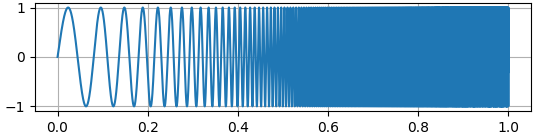
\includegraphics[height=0.8in]{figures/to-replace-two.png}}
\subfloat[Inverse filter $f(t)$ from $x(t)$.]{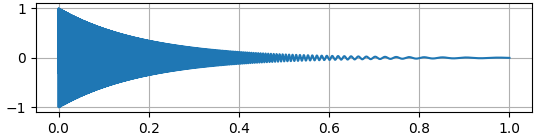
\includegraphics[height=0.8in]{figures/to-replace-three.png}}
\caption{A graph of (a) the Logarithmic Sinusoid Sweep and (b) its inverse.}
\end{figure}

\section{Results of a Sinusoid Sweep}

In practice, tools are available that calculate the inverse filter based on the impulse response. To accomplish this, raw audio files were processed with ReaVerb - a VST application included with Reaper. This program allows for impulse response generation by providing the raw audio and the original impulse, automatically generating the inverse filter. Through this program, the following impulse response was generated from the raw audio:

\begin{figure}[h] % [h] used to prevent {figure} from doing weird positioning
	\begin{center}
		\fbox{
		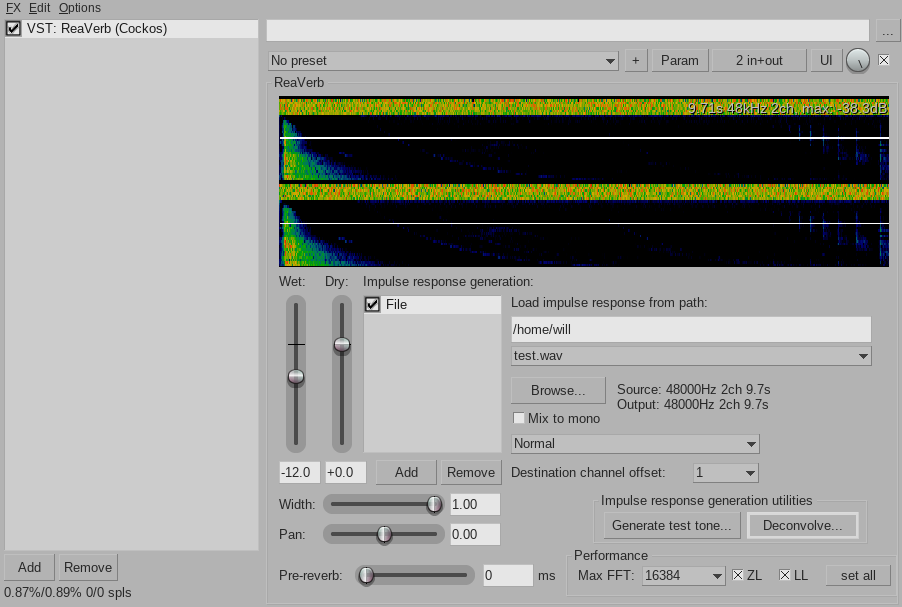
\includegraphics[width=14cm]{figures/Deconvolved.png}
		}
		\caption{A screenshot of the Impulse Response of Gault via Reaverb.}
	\end{center}
\end{figure}

Viewing the IR as a function of time does not reveal much.

\begin{figure}[h] % [h] used to prevent {figure} from doing weird positioning
	\begin{center}
		\fbox{
		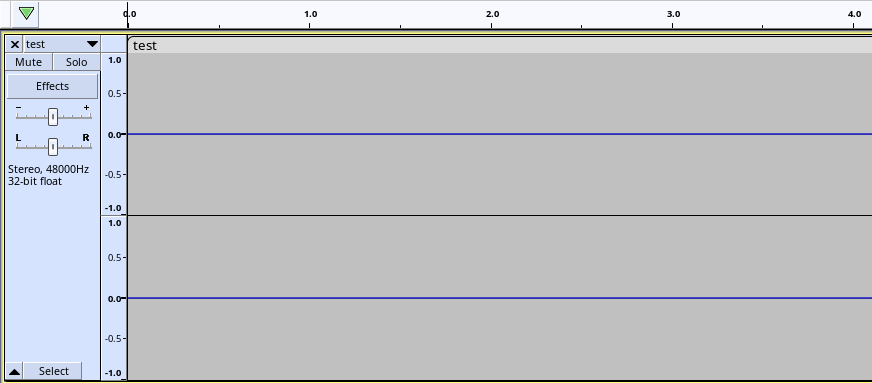
\includegraphics[width=9cm]{figures/time-domain.png}
		}
		\caption{A screenshot of the Impulse Response as a function of amplitude and time.}
	\end{center}
\end{figure}

However, by normalizing the audio output, one is able to clearly see the impulse response.

\begin{figure}[h] % [h] used to prevent {figure} from doing weird positioning
	\begin{center}
		\fbox{
		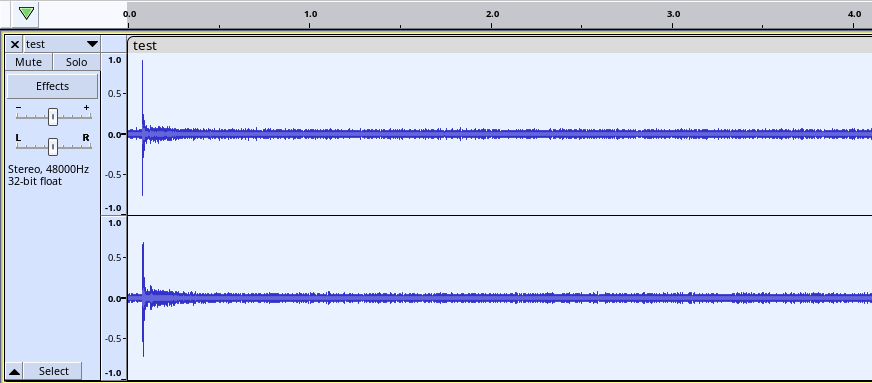
\includegraphics[width=9cm]{figures/normalized.png}
		}
		\caption{The IR normalized.}
	\end{center}
\end{figure}

Some may notice in Figures 5.2 and 5.4 that there appears to be unwanted noise in the IR. By applying a lowpass filter at approximately 17 kHz, this noise is removed.

\begin{figure}[h] % [h] used to prevent {figure} from doing weird positioning
	\begin{center}
		\fbox{
		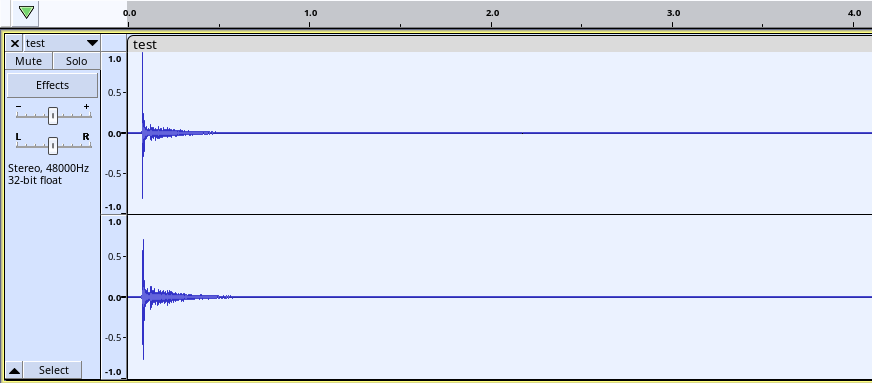
\includegraphics[width=9cm]{figures/lowpass.png}
		}
		\caption{The IR normalized and filtered.}
	\end{center}
\end{figure}
Lastly, the audio file is then cropped to remove areas of silence. Viewing the Impulse Response's amplitude with regard to dB, the resulting $RT_{60}$ time is within 15\% of the predicted value at approximately 1.05s:
\begin{figure}[h]
\begin{center}
\subfloat[The IR cropped.]{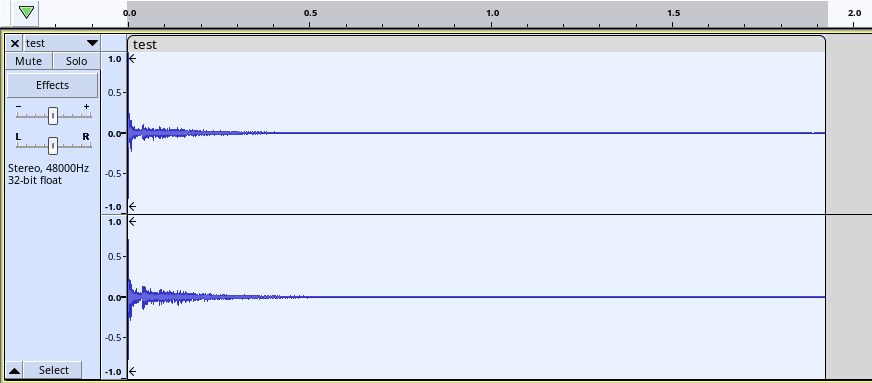
\includegraphics[height=1.2in]{figures/cropped.png}} \hspace*{1.15cm}
\subfloat[The IR with regard to dB.]{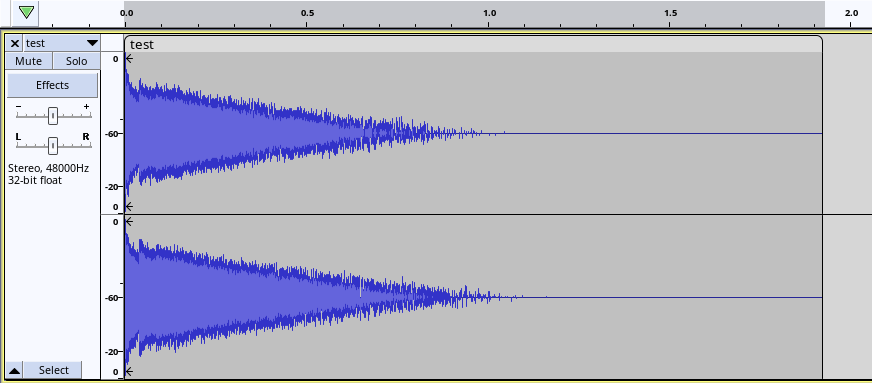
\includegraphics[height=1.2in]{figures/dB-result.png}}
\caption{The IR as a function of (a) its amplitude with respect to time and (b) its dB with respect to time.}
\end{center}
\end{figure}
